% !TEX root=./../maha-dip-notes.tex
\section{Histogram Equalization}

Histogram equalization is a method to adjust image intensities to enhance contrast. The histogram of an image is "flattened" (equalized), redistributing pixel values as uniformly as possible over the intensity range.\cite{stathaki2014histeq}
\subsection{Histogram Equalization (HE)}
\dfn{Histogram Equalization}{A point-wise image transformation that remaps the intensity distribution so that the output histogram is (approximately) uniform. This increases the dynamic range and enhances global contrast.}

\paragraph{For a Continuous Gray Scale Image}, consider gray levels as continuous random variables $ r $ (original) and $ s $ (transformed), with probability density functions (PDFs) $p_r(r)$ and $ p_s(s) $. The transformation $T$ is given by
$$
s = T(r) = \int_0^r p_r(k)\;dk
$$

where the transformation $T$ is monotonically increasing in the range $ 0 \le r \le L-1$ and there exists a one to one mapping from $r$ to $s$ if T is strictly monotonically increasing in the range $ 0 \le r \le L-1$. This condition guarantees that ordering of the output intensities will follow the ordering of the input intensities.\\

Consider a minimal increment of the original intensity r to the intensity $r +
dr$. The intensity $r + dr$ is mapped to an intensity $s + ds$ through the
transformation $T(r)$. Since $T(r)$ is (monotonically) increasing we can easily say that $s + ds \ge s$. All values of the original intensity which are within the interval $[r, r + dr]$ will be mapped to new values within the interval $[s, s + ds]$. Thus, $$\text{Probability}(r \le \texttt{original intensity} \le r + dr)=\text{Probability}(s \le \texttt{new intensity} \le s + ds)$$ i.e.,
$$
    \int_{r + dr}^r p_r(k)\;dk = \int_{s + ds}^s p_s(k)\;dk \implies p_r(r)dr = p_s(s)ds
$$
Transformation for the cumulative distribution function (CDF) is given as 
$$
s = T(r) = (L-1) \int_0^r p_r(k)\;dk
$$
as $p_r(r)dr = p_s(s)ds$, we have $$p_s(s) = \frac{p_r(r)}{\frac{ds}{dr}}$$
From transformation we have $\frac{ds}{dr} = (L-1)  \frac{d}{dr} \int_0^r p_r(k)\;dk = (L-1) p_r(r)$ thus pdf of s is 
$$p_s(s) = \frac{p_r(r)}{\frac{ds}{dr}} = \frac{p_r(r)}{(L-1) p_r(r)} = \frac{1}{(L-1)} $$ which is uniformly distributed and thus the transformation is Histogram Equalization.
\paragraph{For a Discrete Gray Scale Image}
with intensities $r$ in $[0, L-1]$ and histogram $h(r)$, where $ r_k $ denote the $ k $-th gray level (for $ k = 0, 1, ..., L-1 $), $ n_k $ the number of pixels at level $ k $, and $ MN $ the total number of pixels. histogram equalization computes a transformation $HE$ as the cumulative distribution function (CDF)
$$
HE(r) = \sum_{k=0}^{r} \frac{h(k)}{MN}
$$
where $MN$ is the total number of pixels.

\dfn{Histogram Equalization Transformation}{
The transformation $s = HE(r)$ maps each input intensity $r$ to an output intensity $s$ so that $s$ is approximately uniformly distributed over $[0, L-1]$. extending continuous form to discrete case, we have
$$
    s = (L-1) \cdot HE(r) = (L-1) \cdot \sum_{k=0}^{r} \frac{h(k)}{MN}
$$
}

\paragraph{Step-by-step Procedure}
\begin{enumerate}
    \item Calculate the histogram $h(r)$ of image intensities.
    \item Normalize to get probability distribution $p(r)$.
    \item Compute cumulative distribution $HE(r)$.
    \item Map each $r$ by $s = (L-1) \cdot HE(r)$.
    \item Replace each $f(x, y)$ with $s$.
\end{enumerate}

\ex{Histogram Equalization Example}{
Consider a $4 \times 4$ image:
$$
\begin{bmatrix}
1 & 3 & 3 & 3 \\
2 & 3 & 2 & 1 \\
2 & 3 & 2 & 1 \\
1 & 3 & 3 & 3
\end{bmatrix}
$$
Calculate $h(r)$, $T(r)$, and remap all values using $s = (L-1)T(r)$ for $L = 8$. This leads to expanded dynamic range and visually improved contrast.\\

\textbf{Solution:}\\

Possible intensities: $r \in \{1,2,3\}$, but $L=8$ ($0$ to $7$).\\
\textbf{Step 1: Compute $h(r)$ (histogram count)}
\begin{align*}
h(1) &= 4 \\
h(2) &= 4 \\
h(3) &= 8 \\
h(\text{others}) &= 0
\end{align*}
Total pixels: $M \times N = 16$

\textbf{Step 2: Compute normalized histogram $p_r(r)$}
\[
p_r(r) = \frac{h(r)}{16}
\]
\begin{align*}
p_r(1) &= 0.25 \\
p_r(2) &= 0.25 \\
p_r(3) &= 0.5 \\
p_r(0),p_r(4\ldots7) &= 0
\end{align*}

\textbf{Step 3: Compute cumulative distribution $T(r)$}
\[
T(r_k) = \sum_{j=0}^k p_r(r_j)
\]
Assign $r_0=0,\, r_1=1,\, r_2=2,\, r_3=3,\ldots,r_7=7$:

\begin{align*}
T(0) &= p_r(0) = 0 \\
T(1) &= p_r(0) + p_r(1) = 0 + 0.25 = 0.25 \\
T(2) &= T(1) + p_r(2) = 0.25 + 0.25 = 0.5 \\
T(3) &= T(2) + p_r(3) = 0.5 + 0.5 = 1.0 \\
T(4\text{-}7) &= 1.0
\end{align*}

\textbf{Step 4: Remap each value using $s(r) = (L-1)T(r)$}

Since $L=8$,
\[
s(r) = 7 \times T(r)
\]
So,
\begin{align*}
s(0) &= 7 \times 0 = 0 \\
s(1) &= 7 \times 0.25 = 1.75 \rightarrow 2 \\
s(2) &= 7 \times 0.5 = 3.5 \rightarrow 4 \\
s(3) &= 7 \times 1.0 = 7 \\
s(4\text{-}7) &= 7
\end{align*}

\textbf{Step 5: Build remapped image}

\[
\begin{bmatrix}
1 & 3 & 3 & 3 \\
2 & 3 & 2 & 1 \\
2 & 3 & 2 & 1 \\
1 & 3 & 3 & 3
\end{bmatrix}
\longrightarrow
\begin{bmatrix}
2 & 7 & 7 & 7 \\
4 & 7 & 4 & 2 \\
4 & 7 & 4 & 2 \\
2 & 7 & 7 & 7
\end{bmatrix}
\]

\textbf{Summary Table:}

\[
\begin{array}{|c|c|c|c|}
\hline
r & h(r) & T(r) & s(r)\ (\text{rounded}) \\
\hline
0 & 0 & 0.00 & 0 \\
1 & 4 & 0.25 & 2 \\
2 & 4 & 0.50 & 4 \\
3 & 8 & 1.00 & 7 \\
4 & 0 & 1.00 & 7 \\
5 & 0 & 1.00 & 7 \\
6 & 0 & 1.00 & 7 \\
7 & 0 & 1.00 & 7 \\
\hline
\end{array}
\]

\textbf{Result:}
The new image has its intensities spread over the full dynamic range ($0$ to $7$), significantly increasing perceived contrast, which can be seen in the below Figure \ref{hist_eq}.


\begin{figure}[H]
    \centering
    \begin{minipage}{0.45\linewidth}
        \centering
        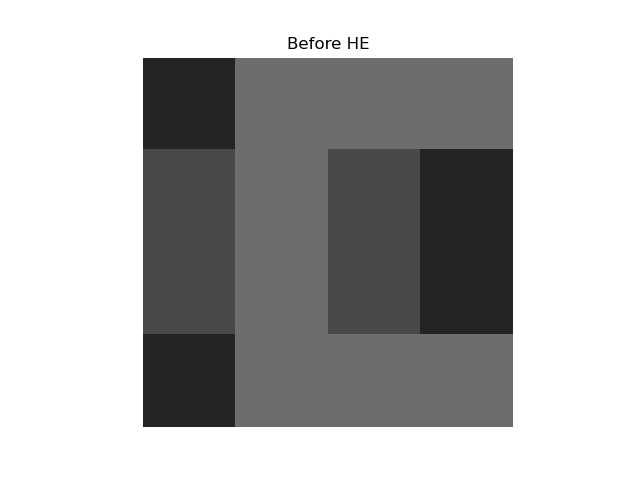
\includegraphics[width=\linewidth]{lec02/Before_HE.png}
        \caption{Original Image}
    \end{minipage}
    \hfill
    \begin{minipage}{0.45\linewidth}
        \centering
        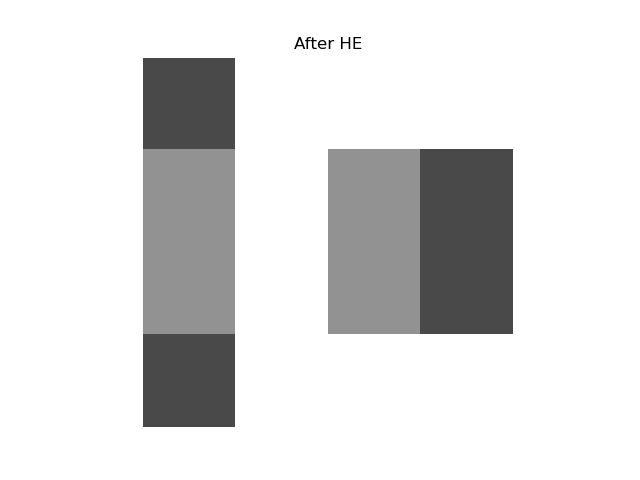
\includegraphics[width=\linewidth]{lec02/After_HE.png}
        \caption{After Histogram Equalization}
    \end{minipage}
    \label{hist_eq}
\end{figure}

}
\paragraph{Advantages of Histogram Equalization}
\begin{itemize}
    \item Enhancement of images with poor contrast.
    \item Preprocessing for computer vision tasks.
    \item Medical imaging, remote sensing.
\end{itemize}
\nt{Histogram equalization may produce undesirable artifacts if the histogram contains large peaks or is multimodal; local methods may better preserve detail.}

\subsection{Adaptive Histogram Equalization (AHE)}

\dfn{Adaptive Histogram Equalization (AHE)}{A technique where histogram equalization is applied locally to small overlapping regions (tiles) of an image, rather than globally, in order to enhance local contrast and bring out more detail in subregions.}

\paragraph{Mathematical Formulation}

Let the image be divided into small regions (tiles) indexed by \( i \). For each tile, compute the local histogram \( h_i(r) \) and local cumulative distribution function (CDF),
\[
HE_i(r) = \sum_{k=0}^{r} \frac{h_i(k)}{M_i N_i}
\]

where \( M_i N_i \) is the number of pixels in tile \( i \).\\

\noindent The local gray levels are then transformed by
\[
s_i = (L-1) \cdot HE_i(r)
\]

for all pixels \( r \) in tile \( i \).\\

To avoid boundary artifacts and ensure smooth transitions, bilinear interpolation is used to combine the mappings of neighboring tiles.

\nt{
\begin{itemize}
    \item Enhances contrast adaptively per local region.
    \item Useful in images with varying illumination.
    \item May amplify noise in relatively homogeneous regions due to over-enhancement.
\end{itemize}
}

\subsection{Contrast Limited Adaptive Histogram Equalization (CLAHE)}

\dfn{Contrast Limited Adaptive Histogram Equalization (CLAHE)}{An improved AHE method that limits the contrast enhancement to avoid noise amplification by clipping the local histogram at a predefined threshold (clip limit).}

\paragraph{Mathematical Formulation}

For each tile \( i \), compute the histogram \( h_i(r) \). Clip the histogram at a clip limit \( C \), redistributing excess pixels equally among all bins to maintain total histogram count
\[
h_i^{clip}(r) = \min(h_i(r), C)
\]
Now, Compute the clipped CDF,
\[
HE_i^{clip}(r) = \sum_{k=0}^{r} \frac{h_i^{clip}(k)}{M_i N_i}
\]
then map pixel intensities in tile \( i \) by
\[
s_i^{clip} = (L-1) \cdot HE_i^{clip}(r)
\]
Finally Combining tiles using bilinear interpolation for smooth transitions results in the final CLAHE image.

\nt{
\begin{itemize}
    \item Controls noise amplification typical in standard AHE.
    \item Provides better visual quality, especially for images with large homogeneous regions.
    \item Widely used in medical imaging, remote sensing, and other applications requiring improved local contrast with controlled noise.
\end{itemize}
}

\subsection{Histogram Matching (Specification)}

We have mapped an image to a uniformly distribution of gray levels, i.e., Histogram Equalization, but in general if need to map it to some other distribution, e.g., a Gaussian distribution, or a distribution that matches another image, then we perform {\it Histogram Matching}, allowing control over the output image appearance beyond simple equalization. Also known as histogram specification or histogram remapping, it's commonly used in image normalization, look adaptation in film, remote sensing for compensating illumination differences.

\dfn{Histogram Matching}{A process to transform an image's histogram to resemble a specified target histogram, useful for standardizing brightness and contrast between images.}

Given an input image $I$ with gray levels \( r \in [0, L-1] \) with probability distribution \( p_r(r) \) and target desired histogram with gray levels \( z \in [0, L-1] \) and distribution \( p_z(z) \).\\
\textbf{Steps:}
\begin{enumerate}
  \item Compute the CDF of the input image,
  \[
  P = P(r) = \sum_{k=0}^{r} p_r(r_k)
  \]    
  
  \item Compute the CDF of the target histogram,
  \[
  Q = Q(z) = \sum_{k=0}^{z} p_z(z_k)
  \]
  
  \item Find the inverse mapping of the target CDF, \( Q^{-1} \), such that for each \( k \in [0,1] \),
  \[
  z = Q^{-1}(s) = \arg \min_z |Q(z) - k|
  \]
  
  \item The overall transformation from the input gray level \( r \) to the output gray level \( z \) is then
  \[
  z = Q^{-1}(T(r))
  \]
\end{enumerate}

This remaps the intensity levels of the input image so its histogram approximately matches the target histogram.

\paragraph{Discrete Case}

For discrete gray levels and histograms \( h_r(r_k) \) and \( h_z(z_k) \), normalized by the total number of pixels \( MN \):

\[
P(r_k) = \sum_{j=0}^k \frac{h_r(r_j)}{MN}, \quad
Q(z_k) = \sum_{j=0}^k \frac{h_z(z_j)}{MN}
\]

Find \( z_k \) such that

\[
z_k = \arg \min_{z} |Q(z) - P(r_k)|
\]

\paragraph{Algorithm}
\begin{enumerate}
  \item Compute histogram and CDF \( P \) of input image.
  \item Compute desired histogram and CDF \( Q \).
  \item For each input gray level \( r_k \), find \( z_k = Q^{-1}(P(r_k)) \) by searching \( Q \).
  \item Replace each pixel value \( r_k \) by \( z_k \).
\end{enumerate}

\nt{Histogram matching is essential in applications where uniformity across image datasets is required, such as medical or satellite image analysis.}

\subsubsection{Additional Theories and Extensions}

\paragraph{Retinex Theory}
Retinex posits that the perceived color of a pixel ($I$) is the product of the light source ($L$) and the reflectance ($R$):
$$
I(x, y) = L(x, y) \cdot R(x, y)
$$
Retinex-based algorithms attempt to decompose an image into illumination and reflectance components for improved color constancy and dynamic range.

\paragraph{Dark Channel Prior}
Used in haze removal, the \emph{dark channel prior} exploits the property that in most non-sky patches of outdoor images, at least one color channel has very low intensity:
$$
\text{dark}(x, y) = \min_{c \in \{r,g,b\}} \left( \min_{(i, j) \in \Omega(x, y)} I^c(i,j) \right)
$$
where $\Omega$ is a local patch. This prior helps estimate atmospheric light and transmission map for dehazing.

\nt{Retinex and dark channel prior are advanced theories, bridging classical image processing and physics-based models for real-world improvements.}

\paragraph{Deep Learning Approaches}

Recent methods leverage deep learning to adapt intensity transformations, contrast normalization, or even build custom histogram-equalization-like layers in neural networks\cite{szeliski2010,govindjee2007,bovik2019,gonzalez2008}.

Deep networks can be trained to perform sophisticated global and local contrast adjustments based on task-specific criteria, outperforming traditional fixed algorithms in complex scenarios.
